\section{API}

A \textit{Web} API é composta por 2 módulos principais (API e Service) e um conjunto de módulos auxiliares. Enquanto que a API lida com pedidos e respostas HTTP e o \textit{Service} é responsável por implementar a lógica do sistema, existem ainda os repositórios (sendo que cada um se responsabiliza por implementar a sua própria lógica de acesso à base de dados) e o índice de imagens (responsável por tratar todas as operações associadas às mesmas).

\begin{figure}[h]
	\centering
	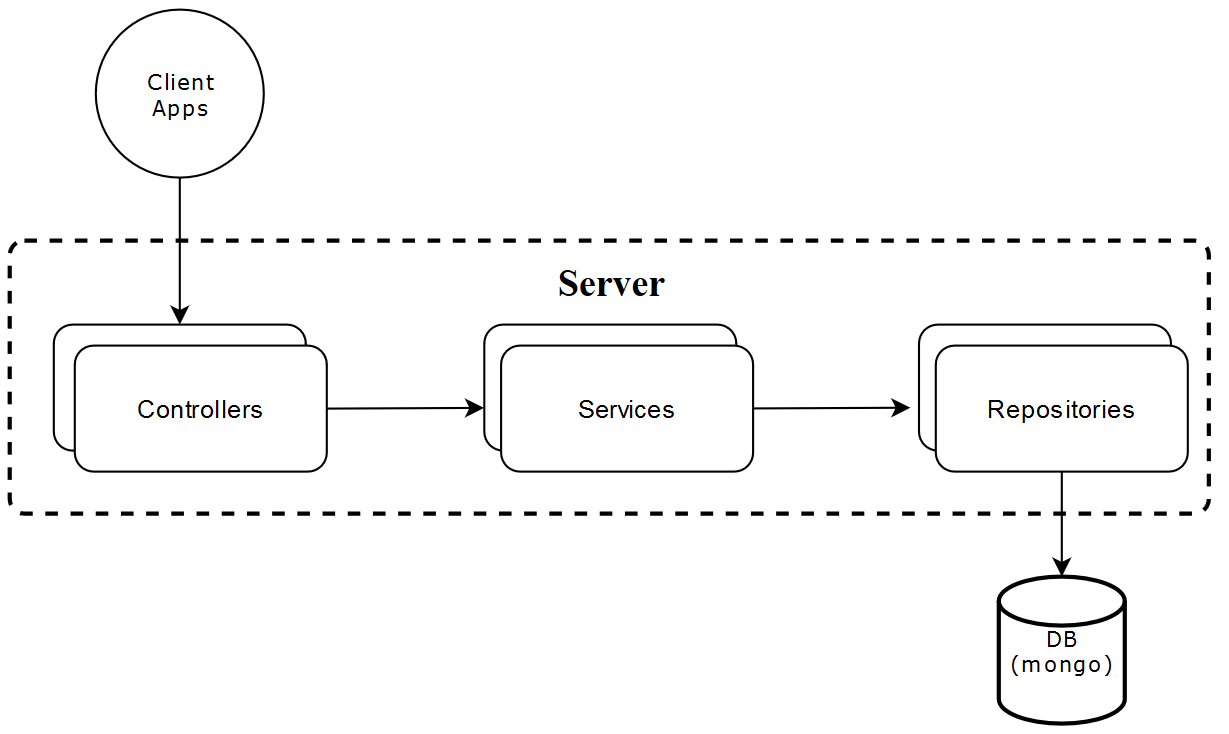
\includegraphics[scale=.50]{api_architeture}
	\caption{Diagrama de arquitetura da API}
\end{figure}

\subsection{API}
Este módulo é responsável por definir os endpoints e lidar com a receção e envio dos pedidos/respostas HTTP. Cada endpoint tem associada uma função que é executada que efetua à chamada ao serviço adequada para realizar a operação solicitada pelo utilizador. \par \medskip

Na próxima página, encontra-se a tabela das operações possíveis de efetuar na API. Refere-se também o método e o URL do pedido a efetuar. Estes pedidos encontram-se também definidos na wiki do projeto. \par \medskip

É de notar que todos os pedidos definidos têm o preâmbulo \textit{/api} e que os que começam por \textit{/auth} necessitam de autenticação prévia por parte do cliente da API. \par \medskip

\newpage

\begin{figure}[h]
	\centering
	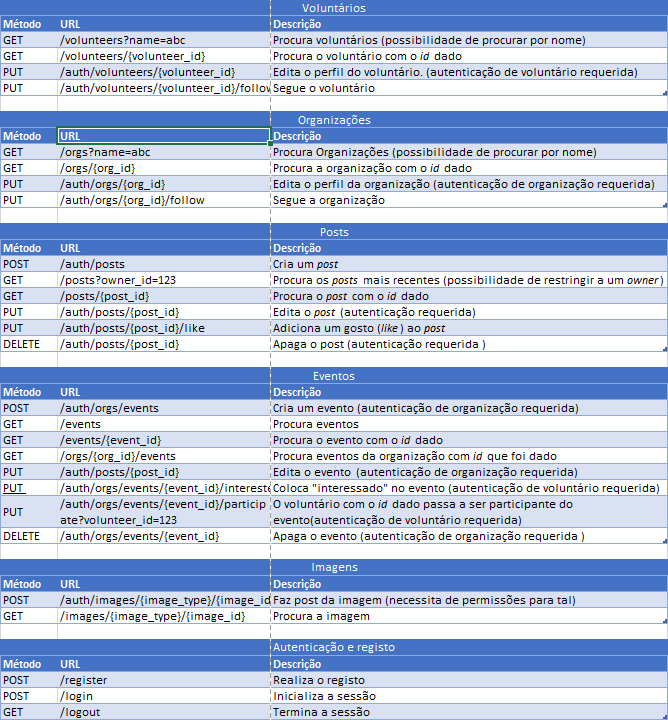
\includegraphics[scale=.70]{endpoints_table}
	\caption{Lista de \textit{endpoints}}
\end{figure}

Para além das funções já referidas, são também definidos (e utilizados) \textit{middlewares} nesta camada de maneira a garantir o cumprimento da necessidade de autenticação aquando de certas operações. A API é ainda responsável por transformar os paramêtros dados pelo cliente através do \textit{URL}, da \textit{query string} e do \textit{body} do \textit{request} (e do objecto sessão quando aplicável) para objetos conhecidos pelo \textit{serviço}. \medskip

\newpage

\subsection{Serviço}
O módulo \textit{Service} cumpre a função de implementar a lógica da aplicação, isto é, garantir que as operações chamadas a partir da API se materializem em mudanças no modelo deste componente, seja a nível de base de dados ou tratamento de operações relativamente às imagens, entre outros. \par \medskip

Este módulo tem as seguintes responsabilidades:
\begin{itemize}
	\item Verificar a validade dos paramêtros fornecidos pela API;
	\item Executar as chamadas necessárias ao módulos adjacentes (\textit{repositories} e \textit{pictures}) de maneira a cumprir a operação solicitada (quer esta seja a inserção em base de dados ou a recolha de informações para verificar a lógica necessária);
	\item Implementar a lógica da aplicação, isto é, quando necessário, efetuar as verificações necessárias e gerar os objectos a colocar/alterar na base de dados.
\end{itemize}

\subsection{Repositórios e acesso a base de dados}
Para cada índice na base de dados, existe uma variação de implementação de \textit{Repository}. Estas implementações fornecem métodos alterados para inserir/modificar/apagar entradas dos índices aos quais se referem. Estes repositórios, por sua vez, têm acesso a uma instância de \textit{BaseRepository} gerada especificamente para si (isto é, inicializada dando parâmetros personalizados consoante o índice). \par \medskip

\textit{BaseRepository} é uma infra-estrutura implementada de maneira a ser genérica para todos os índices e que fornece implementações das típicas operações CRUD como também a possibilidade de gerar os índices de pesquisa necessários para efetuar pesquisas por valor de campos nas tabelas. \par \medskip

\subsection{Base de Dados}
O motor de base de dados escolhido foi o MongoDB. Este segue o padrão \textit{noSQL}, isto é, apresenta um modelo não relacional, tipicamente utilizado no desenvolvimento de redes sociais, devido aos seguintes aspetos:

\begin{itemize}
	\item flexibilidade. Dado em conta que este tipo de plataformas customa ter um crescimento exponencial, a adição de novas features é constante. Num modelo SQL, por vezes é dispendido tempo de implementação a efetuar estas alterações, algo que não é necessário neste caso porque os documentos não têm um esquema fortemente definido, e pode ser inseridos dinamicamente (dois documentos com características diferentes podem ser inseridos no mesmo índice).
	\item integração com Javascript. Os documentos inseridos nesta base de dados têm um formato JSON, algo que se integra facilmente com esta tecnologia.
\end{itemize} 

\subsection{Autenticação}
A componente autenticação deste módulo foi desenvolvida através da ferramente Passport.js. Esta é tipicamente utilizada em conjunto com Express e permite a fácil implementação do conceito sessão através do uso de \textit{cookies}. \par \medskip

Aquando do pedido de autenticação bem sucedido por parte de um cliente da API, são guardadas um conjunto de características identificadoras da sessão do mesmo para que se possa personalizar a sua experiência, e neste caso, permitir ao mesmo que possa fazer \textit{upload} de imagens, criar um \textit{post}, entre outros. \par \medskip

\subsection{Imagens}
De maneira a implementar na sua totalidade um conceito de rede-social a este aplicação, é permitido o upload de imagens para esta plataforma. Estas são divididadas por índices, consoante a sua classe (aquilo que elas referem) e guardadas. \par \medskip

O \textit{upload} de imagens para esta plataforma é apenas possível para utilizadores autenticados, no entanto, o \textit{download} das mesmas é possível a qualquer cliente da API.

\subsection{Paginação e limitação de resultados}
Todos as operações da API que tenham como resultado um conjunto de entidades (por exemplo, um conjunto de \textit{posts}), retornam por omissão um número fixo de resultados. Contudo, a nossa API suporta paginação e \textit{skipping} (isto é, "saltar" resultados) através dos paramêtros \textit{limit} e \textit{skip} da \textit{query string}.

\subsection{Dados e imagens de utilizadores}
Dada a natureza deste projeto, todos os dados (perfis/fotos/\textit{posts}) serão públicos para todos, e como tal, aquando do registo nas aplicações cliente, os utilizadores das mesmas serão sensilibizados relativamente à visibilidade dos seus dados.

\subsection{Documentação e definição da API}
Toda a documentação sobre as regras e indicações relativamente à utilização desta API encontram-se na \textit{wiki} do repositório do projeto, sendo que o acesso será avaliado quando solicitado aos autores. Esta \textit{wiki} contém informações relativamente à definição mais explícita dos endpoints, erros, entre outros.